\documentclass[11pt, oneside]{article}   	% use "amsart" instead of "article" for AMSLaTeX format
\usepackage{geometry}                		% See geometry.pdf to learn the layout options. There are lots.
\geometry{letterpaper}                   		% ... or a4paper or a5paper or ... 
%\geometry{landscape}                		% Activate for rotated page geometry
%\usepackage[parfill]{parskip}    		% Activate to begin paragraphs with an empty line rather than an indent
\usepackage{graphicx}				% Use pdf, png, jpg, or eps§ with pdflatex; use eps in DVI mode
								% TeX will automatically convert eps --> pdf in pdflatex		
\usepackage{amssymb}
\graphicspath{{/Users/ananyarao/Desktop/AI_ML/ai_ml_pictures/}}
%SetFonts

%SetFonts


\title{ARTIFICIAL INTELLIGENCE FOUNDATIONS: MACHINE LEARNING}
\author{Ananya Rao}
%\date{}							% Activate to display a given date or no date

\begin{document}
\maketitle
\pagebreak
\tableofcontents
\pagebreak
\section{WHAT IS MACHINE LEARNING?}
\subsection{What it means to learn?}
\begin{itemize}
\item Moving away from explicit instructions, instead give the computer the data and tools it needs to study and solve problems.
\item Should also have the ability to remember and adapt, evolve and learn.
\item Start small -- go big.
\item In humans : You have a problem -- so you form a rule -- Apply rule -- wait for feedback -- Adjust rule if needed.
\item In computers : Start by testing with small data first -- then use statistical algorithms to see how the data fits together 
\item Anytime a computer learns something new, it adds it to its memory so it can improve and adapt.
\end{itemize}
\subsection{Work with Data}
\begin{itemize}
\item Example Scenario where Machine Learning can be used : \\
You need to write a Program that detects spam messages that are filled with unwanted Ads and Viruses.\\
You could write an algorithm that searches for certain words (eg. Gold, Lottery, Winner) within the messages and simply deletes them. \\
However, this is not a bulletproof algorithm and is easy to spoof. Eg. Replace O's with zeroes, or just use images.\\
Many non-spam messages might also be deleted based on these parameters. \\
\item To use the machine learning approach -> you first want to split your data between "training data" and "test data".
\item The training data is a smaller chunk that you use to find patterns.
\item With our spam message problem :
We can first take 10,000 emails as our training data set. We use this to build and refine our model before we test on it our test data which has over a million messages. \\
\item BINARY CLASSIFICATION is often used in such scenarios. Binary classification in our example would lead to dividing messages into spam and regular emails. 
\item The machine decides if messages are spam or not by grouping words likely to be found in spam messages. Then it gives a score which portrays the likelihood that the message is spam.
\item Once you have an ML algorithm, you tune the necessary hyper parameters to make an accurate prediction.
\item REMEMBER: Even though it is the programmer that inputs the data, chooses the Algorithm and makes necessary adjustments, it is indeed the machine that makes the fundamental decision of whether a message is spam or not.
\end{itemize}
\subsection{Apply machine learning.}
\begin{itemize}
\item It is easy to collect massive amounts of data, but it is hard to get insight from this collected data. This is where machine learning comes in.
\item Example : Recommended Videos based on the videos you usually watch, Customized search results based on previous searches.
\item In ML, you are using AI to help your program find patterns in massive datasets. Most of these patterns may never be detected by humans. 
\item TIP : Before you start on your machine learning project, you have to think about your data. Is it high quality, do you have enough data? , etc.
\item Think about the best strategies to get high quality and diverse data sets.
\end{itemize}
\subsection{Different types of machine learning}
\begin{itemize}
\item The most important aspect of ML is the process of "Learning". What strategies must one use to learn something new? 
\item Example : You want to learn Chess. \\
You could :\\ 
1. Hire a chess Tutor : They would introduce you to the specifics and rules of the game. You could practice by playing against the tutor who would supervise your moves. \\
2. You could also go to public parks and watch multiple experts play the game. However you could not ask them questions. You might be able to understand the game and some strategies in lieu of your numerous hours of observations.\\
3. You might even try a combination of both of these approaches. The tutor gives you the specifics and rules -- and you use your observation skills to watch expert players and see new strategies to approve.
\item These strategies are very similar to how a machine might learn.
\item SUPERVISED LEARNING : The Data Scientist acts like a tutor for the machine. They train the machine by giving it specific rules and an overall strategy.
\item UNSUPERVISED LEARNING: You have the machine make all the observations on its own. The machine might not know names and labels but they'll find patterns on their own.
\item SEMI-SUPERVISED LEARNING : A mix of supervised and unsupervised learning. Here, the data scientist trains the machine just a little bit so its gets a high-level overview. Most of the learning about the rules and strategies is through observing different patters.
\item Each learning method has its pros and cons.
\item For supervised learning : you must have a knowledgable tutor.
\item For unsupervised learning: You need to have access to a lot of data. The quality of the data is also a factor.
\item With semi-supervised learning: You can run into trouble on both sides.
\item Many a time, we use the learning methods depending on the things you have access to.
\end{itemize}
\section{DIFFERENT WAYS A MACHINE LEARNS}
\subsection{Supervised}
\begin{itemize}
\item In this type of learning, you show the machine the connection between different variables and known outcomes.
\item In ML, the variables are referred as LABELED DATA snd outcomes are referred as OUTPUTS.
\item EXAMPLE : \\
You want to create a program that estimates how long it will take you to drive home. \\
Your approach would be to first create a set of labeled data which would include weather conditions, Time of day, whether its a holiday. These are your inputs. \\
The output would be the commute time.
\item You could use statistics (e.g. regression) and assess how the independent variables affect the dependent variable.
\item  An ML approach to the commute problem : \\
First create a Training Set. \\
Based on this Training Set, your machine might find a direct relationship between variables such as the amount of rain and the commute time. OR the time at which you leave work and the time it takes to reach home.\\
The machine begins to understand how weather and time of the day affects commute time. \\
\bigskip 
Next, The machine takes the training set and applies it to a test set of your data. \\
This to ensure that your algorithm holds true even when you're looking at many more days.\\
You should also give your program feedback on how accurate it was in its predictions.\\
\item REMEMBER : In supervised learning, you know a lot about the Training data.
\item You can feed labeled data into the machine thats easily classified.
\item This classified data is the key difference between supervised learning and the other forms of machine learning.
\end{itemize}
\subsection{Unsupervised}
\begin{itemize}
\item Learning and improving by trial and error is key to unsupervised learning.
\item You do not work with labeled data or show the machine the correct output. 
\item Instead you're using different algorithms to let the machine create connections by studying and observing the data.
\item MULTICLASS CLASSIFICATION : Data sorted into several different groups. 
\item A real world example of multiclass classification : separating candy on halloween based on the ones you like the best.
\item EXAMPLE : Let's say you have a bag of never seen before candy. How do you classify these? 
\item You essentially make your own groups : could make groups based on the Size and Wrapping Color of candies. 
\item Similarly, the machine studies Data and comes up with its own observations.
\item Access to massive amounts of data is necessary for Unsupervised learning.
\end{itemize}
\subsection{Semi-supervised}
\begin{itemize}
\item A combination of supervised and unsupervised learning.
\item EXAMPLE : \\
You want to create a program that translates speech to text. \\
The unsupervised learning method may not be useful in this case as the machine mine cluster words together but has no idea what they mean. \\
Only Supervised learning will not help either as it is too labor intensive to label each sound and their corresponding words. \\
\item One may use semi-supervised learning in this case, you can start with a small training set of very common words and phrases. The machine can use this to create basic classification which is analogous to the training set in supervised learning.
\item Next, you would feed the training set to the machine and let it study and observe the rest of the data. This is similar to unsupervised learning. The machine can now expand its vocabulary based on what it's already classified. This is called INDUCTIVE REASONING.
\item Examples of semi-supervised learning are inductive reasoning and transductive reasoning.
\item Transductive reasoning tries to improve the ML model by guessing what's in the unlabeled data.
\item Inductive and transductive reasoning might lead to greater errors.
\item TIP: Semi-supervised learning only makes sense to use when the other learning methods fail. It is probably not the best method to start with.
\end{itemize}
\subsection{Reinforcement}
\begin{itemize}
\item This type of learning is different from the three discussed before. With the other models, you are trying to find the best model, the one that is most accurate. 
\item Reinforcement learning requires the machine to continuously iterate to improve the outcome.
\item It is extremely open-ended. You are reinforcing the behaviours in which you want the machine to behave. Machines are given "rewards" for completing intended tasks.
\end{itemize}
\subsection{Q-Learning}
\begin{itemize}
\item This is a type of reinforcement learning.
\item Q-Learning consists of set environments or States.
\item There are also possible actions that lead to responses.
\item You want the machine to improve the quality of the outcome represented by the letter Q.
\item EXAMPLE : The game space invaders which has a complex reward system. \\
You start out with Q = 0. Then you want the machine to learn which actions will improve the conditions. Each time an action improved the state of the model, the Q value would increase accordingly.
\item Essentially, the Q goes up based on states and actions.
\item The reiterative aspect of this type of learning is that the machine is allowed to go through endless simulations of actions and states until it finds the best strategy.
\end{itemize}
\section{POPULAR LEARNING ALGORITHMS}
\subsection{Problems that use machine learning}
\begin{itemize}
\item Categories of supervised learning : Binary (yes/no) , multi-class and regression.
\item All binary classification uses supervised learning. You need a developer in the beginning to set parameters.
\item Multi-class classification has multiple outcomes possible.
\item Regression problems tend to have a continuous solution. We look for trends instead of classifying data into different groups. There are no pre-defined outcomes. 
\end{itemize}
\subsection{Decision trees}
\begin{itemize}
\item These can be used for binary classification challenges with supervised machine learning.
\item You can set up predictors and match them with possible outcomes.
\item EXAMPLE : Let's say the problem that we're creating a decision tree for is whether or not someone is likely to go to the beach.
\item We create 3 predictors - Sky, Weekend, and Wind speed.
\item Our outcome variable will be "Yash goes to the beach". This has a binary outcome : He either will or wont.
\item Next, we create a training data set using past information we have about yash.
\bigskip \\
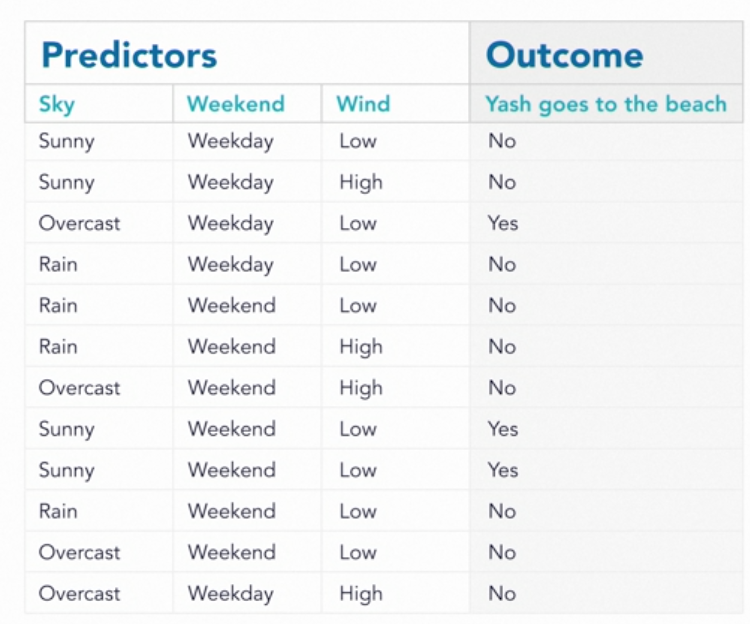
\includegraphics{binary}
\bigskip \\
\item However, this table is not a decision tree. To create a decision tree we must split our data based on our predictors.
\item You must pick a root node predictor. Here we pick Sky.
\bigskip \\
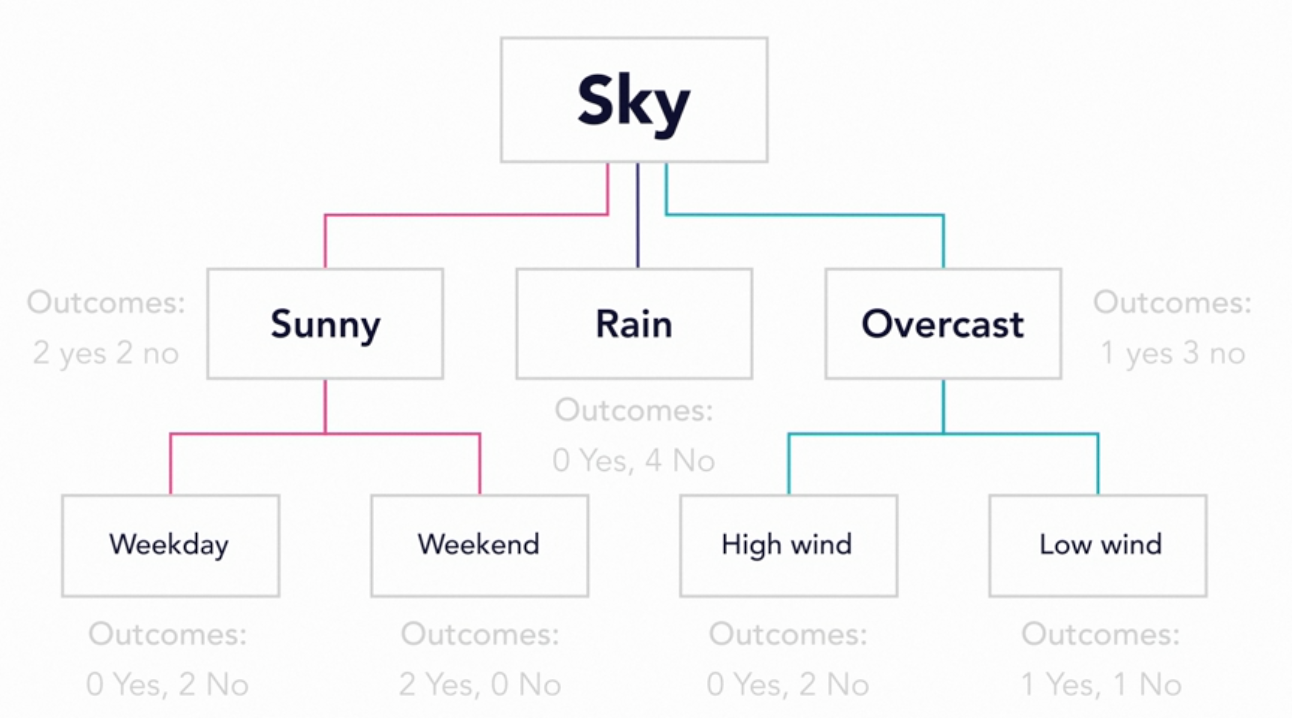
\includegraphics[scale=0.6]{decision_tree}
\bigskip \\
\item Notice that there are no nodes coming from the Rain node. This indicates that there are no outcomes where there's a rainy day and Yash still goes to the beach.
\item Your decision tree must always point towards a binary yes or no outcome. If this is not the case, you might have too much entropy.
\item To get rid of entropy, you must either split with a different predictor or not include some predictors at all.
\end{itemize}
\subsection{k nearest neighbor}
\begin{itemize}
\item This is useful for multi-class classification.
\item It is an instance based algorithm - also called lazy learning, where the bulk of computation happens before you classify data.
\item Learning does not happen continuously and you run all your computation in one big instance.
\item k-NN (k-Nearest neighbour) compares something you don't know to what you already have.
\item k-NN takes a lot of computation problem and is expensive for large data sets.
\item Example : Comparing a dog whose breed you don't know by comparing with pictures of several dog breeds and looking for similar characteristics. We try to classify the dog based on its nearest neighbor.
\item Another way to look at this algorithm is not minimize the distance between the unknown and the known neigbours.
\item The closer you are to your nearest neighbour, the more likely you are to be accurate. 
\item Most common way to do this is using the Euclidean distance formula.
\item EXAMPLE : We decide on two predictors for classifying the breed of our unknown dog : hair length and weight, and create a plot with these factors on the axes.
\item We plot the hair length and weight of the dogs whose breed we know, as well as that of the unknown dog.
\item Taking a k = 5, or five of its closest neighbours and assessing the distance between the points, we can make accurate predictions of the breed.
\bigskip \\
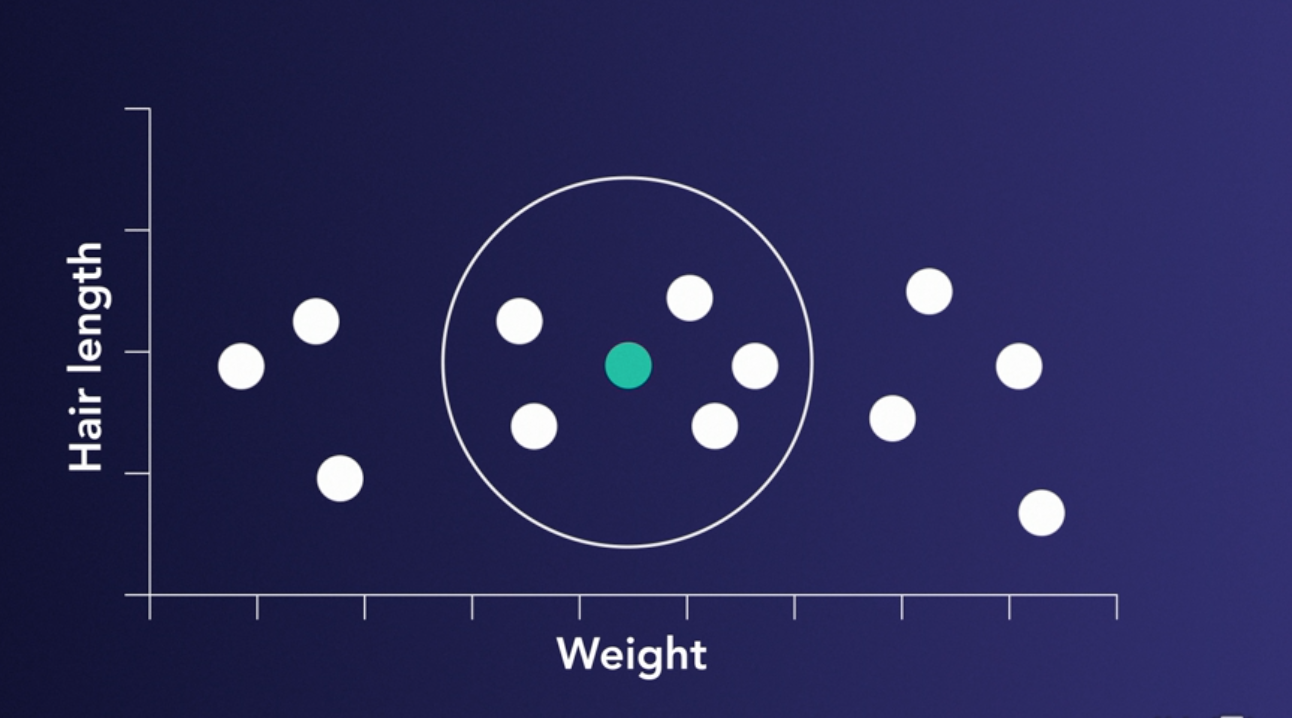
\includegraphics[scale=0.6]{k-NN}
\bigskip \\
\end{itemize}
\subsection{k mean clustering}
\begin{itemize}
\item REMEMBER : This is not the same as the k-NN method.
\item This is an unsupervised ML algorithm.
\item Algorithm runs again and again to select centroids which will represent each cluster.
\item Distance (Variance) between unknown points and these centroids help sort them into clusters.
\item This method is not very effective on outliers.
\end{itemize}
\subsection{Regression}
\begin{itemize}
\item Unlike other methods where lazy learning occurs and the outcome is given in one big splash, regression highlights more of a continuous numerical relationship.
\item Regression analysis looks at the relationship between predictors and your outcome.
\item Regression is less about learning and more about predicting.
\end{itemize}
\subsection{Naive Bayes}
\begin{itemize}
\item RECALL : Supervised learning classifies your data. Unsupervised learning clusters your data.
\item Bayseian algorithm : statistical model based on conditional probability (How one thing affects another)
\item Naive Bayes is one of the most popular ML algorithms. It is called "naive" because it assumes that all predictors are independent from one another.
\item Mostly used for binary or multiclass classification.
\item If we tried to solve the dog classification problem using Bayesian algorithm : We'd select three classes and predictors.
\bigskip \\
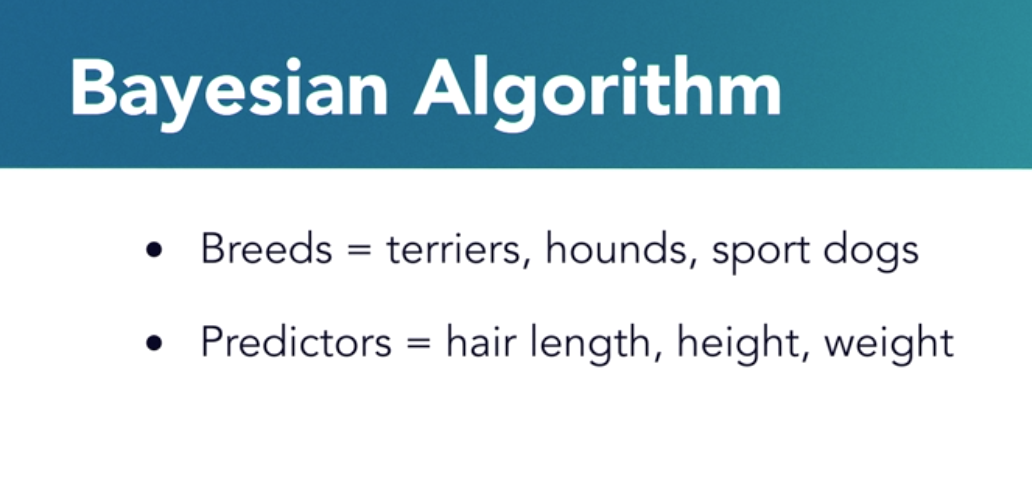
\includegraphics[scale=0.6]{bayesian}
\bigskip \\
\item Note that some of these predictors are autocorrelated. The algorithm considers them to be independent though.
\item Next, the algorithm does something called Class predictor probability where it looks at each independent predictor and estimates the probability of a dog belonging in a particular class based on that predictor.
\item You can use the weighted multiplication algorithm to figure out which probability is the highest.
\bigskip \\
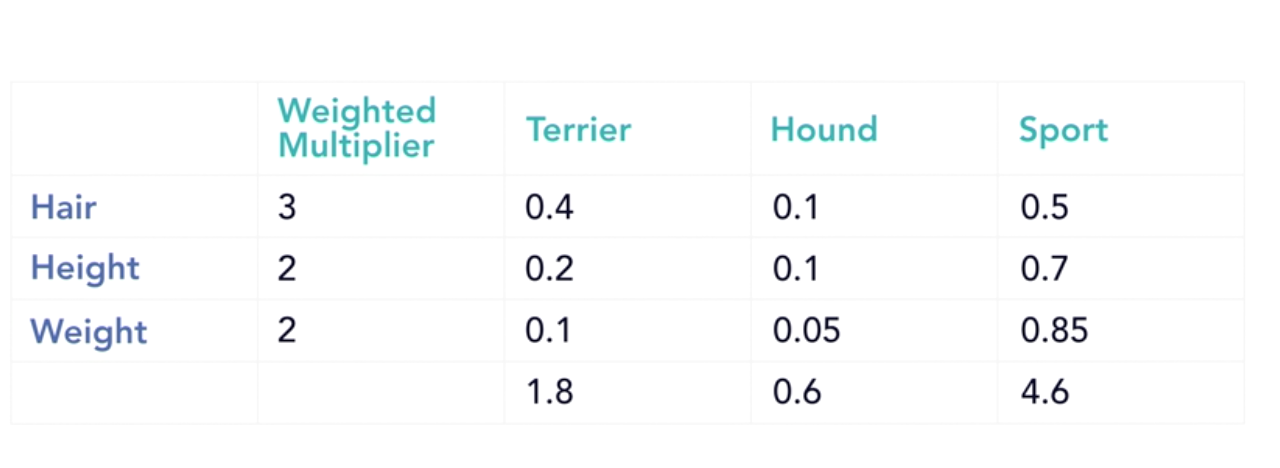
\includegraphics[scale=0.6]{naivE}
\bigskip \\
\end{itemize}
\section{APPLYING ALGORITHMS}
\subsection{Follow the data}
\begin{itemize}
\item We need to be aware of any BIAS or VARIANCE in our data models.
\item Bias is the gap between your predicted value and the actual outcome.
\item Variance is when predicted values are scattered all over the place.
\item High bias / low variance = consistently wrong predictions.
\item High bias/ high variance is worse = consistently wrong predictions in an inconsistent way.
\item An example of low bias and low variance is all arrows fired on a target land in the centre of the bullseye.
\bigskip \\
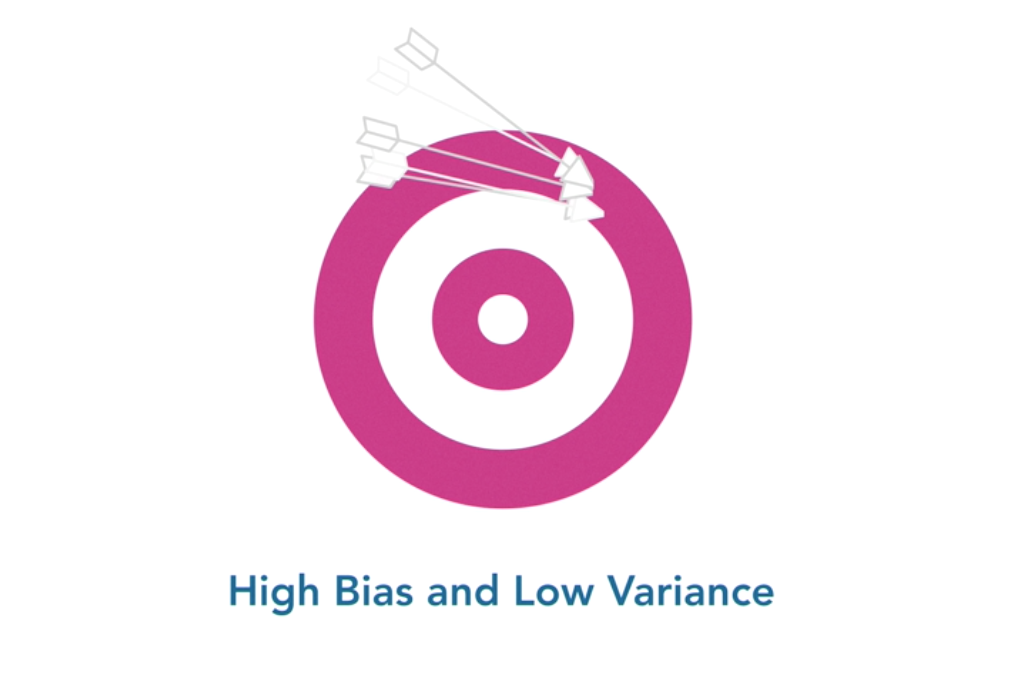
\includegraphics[scale=0.6]{bias}
\bigskip \\
\begin{center} In this example, Because the arrows are away from the bullseye, the bias is high. However all arrows are concentrated around one spot - making the variance low.
\end{center}
\item Based on whether you have too much bias or variance, we use different ML techniques.
\end{itemize}
\subsection{Fit the Data}
\begin{itemize}
\item Example : Creating an Algorithm that predicts the price of a house.
\item We choose 4 predictors : Square footage, Location, Number of baths, Number of beds. The outcome is the value of the house.
\item Your data might have high variance : houses with the same features have drastic price differences. To fix this, you might increase the complexity of your model and add more predictors such as location, view, etc.
\item The added complexity has made the data more flexible, but also more difficult to manage. It will be hard to see relationships between predictors. This is known as OVERFITTING.
\item On the other hand, if less predictors are used in the model this might also cause incorrect predictions. This is known as UNDERFITTING. Low flexibility, but easy to manage.
\item People might often use the terminology of signal and noise : Signal is something that can be used to make accurate predictions while noise might be the natural variances that do not offer any insights.
\item REMEMBER : Look for more signal and less noise in your data.
\end{itemize} 
\subsection{Select the best algorithm}
\begin{itemize}
\item If your data is labeled, you will probably end up picking supervised learning where you know about both - the input and the output.
\item Similarly, if your data is unlabeled, you will end up choosing unsupervised learning where the machine makes its own clusters.
\item If you have lots of unlabeled data, you might end up choosing k-means clustering or some other efficient way to cluster your groups.
\item For lots of labeled data, you can use regression, k-NN or decision trees.
\end{itemize}
\subsection{Ensemble Modeling}
\begin{itemize}
\item Using ensemble modelling, you create different ensembles of ML algorithms.
\item There are three ways to create ensembles - bagging, boosting and stacking.
\item Bagging is when you create several different versions of the ML algorithm. Example : Having multiple decision trees with different predictors at the root node.
\item Boosting is when you use multiple different ML algorithms to boost the accuracy. Example using k mean clustering with decision trees.
\item Stacking is when you use several ML algorithms and stack them to increase the accuracy.
\end{itemize}
\section{MACHINE LEARNING CHALLENGES}
\begin{itemize}
\item The first challenge is making sure that your team asks interesting questions.
\item Second, one must keep training data separate from testing data.
\item Third, Do not spend too much time working with algorithms. Time investment is important.
\end{itemize}
\end{document}  